%-------------------------------------------------------------------------------
%-------------------------------------------------------------------------------
%-------------------------------------------------------------------------------
\chapter{Intégration II : Fourier}
%-------------------------------------------------------------------------------
%-------------------------------------------------------------------------------
{\sf Un problème important lorsque l'on étudie des fonctions est de définir, de manière approchée, une fonction avec un nombre limité de variables. En effet une fonction n'est connue que par sa valeur en tout point d'un intervalle $I$ (souvent $\R$ ou un segment), c'est un nombre infini (même non dénombrable) de variables mais un ordinateur ne peut n'en gérer qu'un nombre fini.

Il existe deux stratégies principales.
\begin{enumerate}
    \item On se restreint à un segment $[a;b]$ qu'on subdivise en plus petit segments $[a_k;a_{k+1}]$ ; sur chacun d'eux on approche la fonction par une fonction {\bf très} simple. Par exemple les valeurs (approchées) des $f(a_k)$ permettent d'approcher $f$ par une fonction affine sur $[a_k;a_{k+1}]$. Si on ajoute la valeur des dérivées on obtient une approximation par les fonctions splines cubiques.
    \item On choisit un type de fonctions considérées comme basiques sur $I$ et on cherche à approcher $f$ par une somme finie de telles fonctions. On utilise des approximations par des polynômes, des polynômes trigonométriques, des ondelettes \dots
\end{enumerate}
\medskip
Dans l'étude des phénomènes périodiques on utilise la décomposition de Fourier : une fonction $T$-périodique est approchée par un polynôme trigonométrique de période $T$ c'est à dire une sommes de fonctions de la forme $t\mapsto \cos(n\omega t)$ et  $t\mapsto \sin(n\omega t)$ avec $\displaystyle \omega = \frac{2\pi}T$.}
%-------------------------------------------------------------------------------
%-------------------------------------------------------------------------------
\section{Définition}
%-------------------------------------------------------------------------------
%-------------------------------------------------------------------------------
On admet que pour une fonction $f$ $T$-périodique et assez régulière\footnote{On admet que ce sera toujours le cas des fonctions envisagées}, les coefficients 
%-------------------------------------------------------------------------------
\begin{enumerate}
    \item $\displaystyle a_0 = \frac 1T\int_{-T/2}^{T/2}f(t)\d t$, la valeur moyenne de $f$
    \item $\displaystyle a_n = \frac 2T\int_{-T/2}^{T/2}\cos(n\omega t)f(t)\d t$  pour $n\ge 1$,     
    \item $\displaystyle b_n = \frac 2T\int_{-T/2}^{T/2}\sin(n\omega t)f(t)\d t$ pour $n\ge 1$
\end{enumerate}
%-------------------------------------------------------------------------------
avec $\displaystyle \omega = \frac{2\pi}T$ permettent approcher $f$ par la somme de Fourier d'ordre $n$

\[S_N(f)(t) =   a_0 + \sum_{n=1}^{N} a_n\cos(n\omega t) + b_n\sin(n\omega t)\]
%-------------------------------------------------------------------------------
%-------------------------------------------------------------------------------
\section{Calculs}
%--------------------------------------------------------------------------
%--------------------------------------------------------------------------
On utilisera les fonctions mathématiques du module \type{math}.
\begin{lstlisting}
from math import *
\end{lstlisting}
%--------------------------------------------------------------------------
%--------------------------------------------------------------------------
\subsection{Intégrales}
%--------------------------------------------------------------------------
%--------------------------------------------------------------------------
\begin{Exercise}\it
Écrire une fonction \type{integrale(f, a, b)} qui calcule qui calcule une valeur approchée de l'intégrale $\displaystyle \int_a^b f(t) \d t$ en utilisant la méthode des trapèzes en découpant l'intervalle en 1000 sous-intervalles de même largeur.
\end{Exercise}
%--------------------------------------------------------------------------
\begin{Answer}
\begin{lstlisting}
def integrale(f, a, b):
    n = 1000
    pas = (b-a)/n
    somme = (f(a) + f(b))/2
    for k in range(1, n-1):
        ak = a + k*pas
        somme = somme + f(ak)
    return somme*pas
\end{lstlisting}
\end{Answer}
%--------------------------------------------------------------------------
%--------------------------------------------------------------------------

On pourra aussi utiliser la fonction de calcul des intégrales du module \type{scipy}
\begin{lstlisting}
from scipy.integrate import quad
\end{lstlisting}
\begin{enumerate}
\item \type{quad(f, a, b)} renvoie un couple $(I, e)$ où $I$ est une valeur approchée de $\displaystyle \int_a^b f(t) \d t$ et $e$ est une estimation de l'erreur commise.
\item  La fonction \type{quad} permet des bornes infinies, \type{inf} de la bibliothèque \type{math} représente $+\infty$.
\end{enumerate}

On peut remplacer la fonction de l'exercice ci-dessus par
%--------------------------------------------------------------------------
\begin{lstlisting}
def integrale(f, a, b):
    I, e = quad(f, a, b)
    return I
\end{lstlisting}
%-------------------------------------------------------------------------------
%-------------------------------------------------------------------------------
\subsection{Coefficients}
%--------------------------------------------------------------------------
%--------------------------------------------------------------------------
Dans le calcul des coefficient on doit intégrer des fonctions différentes pour chaque indice ; on définira une fonction dans le corps d'une fonction.
%--------------------------------------------------------------------------
\begin{lstlisting}
def liste_a(f, N, T):
    ...
    for n in range(1, N+1)
        def fn(x):
            return f(x)*cos(omega*n*x)
        .... # On peut utiliser fn
    return 
\end{lstlisting}
%--------------------------------------------------------------------------
%--------------------------------------------------------------------------
%--------------------------------------------------------------------------
\begin{Exercise}\it
Écrire une fonction \type{liste\_a(f, N, T)} qui calcule la liste des coefficients $a_n$, $0\le n\le N$, de la fonction $f$ périodique de période $T$. On notera qu'on renvoie une liste de taille $N+1$.
\end{Exercise}
%--------------------------------------------------------------------------
\begin{Answer}
\begin{lstlisting}
def liste_a(f, N, T):
    A = [0]*(N+1)
    A[0] =  integrale(f, -T/2, T/2)/T
    omega = 2*pi/T
    for n in range(1, N+1):
        def fn(x):
            return f(x)*cos(omega*n*x)
        A[n] = 2*integrale(fn, -T/2, T/2)/T
    return A
\end{lstlisting}
\end{Answer}
%--------------------------------------------------------------------------
%--------------------------------------------------------------------------
\begin{Exercise}\it
Faire de même pour les coefficients $b_n$, on laissera la valeur 0 pour $b_0$.
\end{Exercise}
%--------------------------------------------------------------------------
\begin{Answer}
\begin{lstlisting}
def liste_b(f, N, T):
    B = [0]*(N+1)
    omega = 2*pi/T
    for n in range(1, N+1):
        def fn(x):
            return f(x)*sin(omega*n*x)
        B[n] = 2*integrale(fn, -T/2, T/2)/T
    return B
\end{lstlisting}
\end{Answer}
%-------------------------------------------------------------------------------
%-------------------------------------------------------------------------------
\subsection{Sommes de Fourier}
%-------------------------------------------------------------------------------
%-------------------------------------------------------------------------------

Pour éviter les calculs répétés, l'évaluation des sommes partielles reçoit en paramètres les listes, de même longueur, des coefficients $a_n$ et $b_n$.
%--------------------------------------------------------------------------
%--------------------------------------------------------------------------
\begin{Exercise}\it
Écrire une fonction \type{somme\_Fourier(A, B, T, x)} qui calcule la somme partielle $\displaystyle  a_0 + \sum_{n=1}^{N} a_n\cos(n\omega x) + b_n\sin(n\omega x)$ où $\omega = \frac{2\pi}T$ et $a_n$ (resp. $b_n$) est la valeur de \type{A[n]} (resp. \type{B[n]}).
\end{Exercise}
%--------------------------------------------------------------------------
\begin{Answer}
\begin{lstlisting}
def somme_Fourier(A, B, T, x):
    N = len(A)
    s = 0
    w = 2*pi/T
    for n in range(N):
        s = s + A[n]*cos(n*w*x) + B[n]*sin(n*w*x)
    return s
\end{lstlisting}
\end{Answer}
%-------------------------------------------------------------------------------
%-------------------------------------------------------------------------------
\section{Visualisations}
%--------------------------------------------------------------------------
%--------------------------------------------------------------------------
Pour afficher le graphe d'une fonction, une méthode possible est la suivante.
\begin{enumerate}
\item On doit avoir importé le module graphique
\begin{lstlisting}
import matplotlib.pyplot as plt
\end{lstlisting}
\item On définit une liste des abscisses pour représenter un intervalle $[a; b]$. Cela peut se faire avec 
\begin{lstlisting}
n = 1000
pas  = (b-a)/n
X = [a + k*pas for k in range(n+1)]
\end{lstlisting}
\item On calcule la liste des images de ces abscisses
\begin{lstlisting}
X = [f(x) for x in X]
\end{lstlisting}
\item On trace le graphe
\begin{lstlisting}
plt.plot(X, Y)
plt.show()
\end{lstlisting}
\item Si on a besoin de tracer les graphes de plusieurs fonctions, on fait un calcul du tracé (\type{plt.plot}) par fonction et o finit par un unique \type{plt.show()}. On peut légender les tracés.
\begin{lstlisting}
plt.plot(X, Y1, label = "Fonction f1")
plt.plot(X, Y2, label= "Fonction f2")
plt.legend()
plt.show()
\end{lstlisting}
\end{enumerate}
%--------------------------------------------------------------------------
%--------------------------------------------------------------------------
\subsection{Signal triangulaire}
%--------------------------------------------------------------------------
%--------------------------------------------------------------------------
\begin{center}
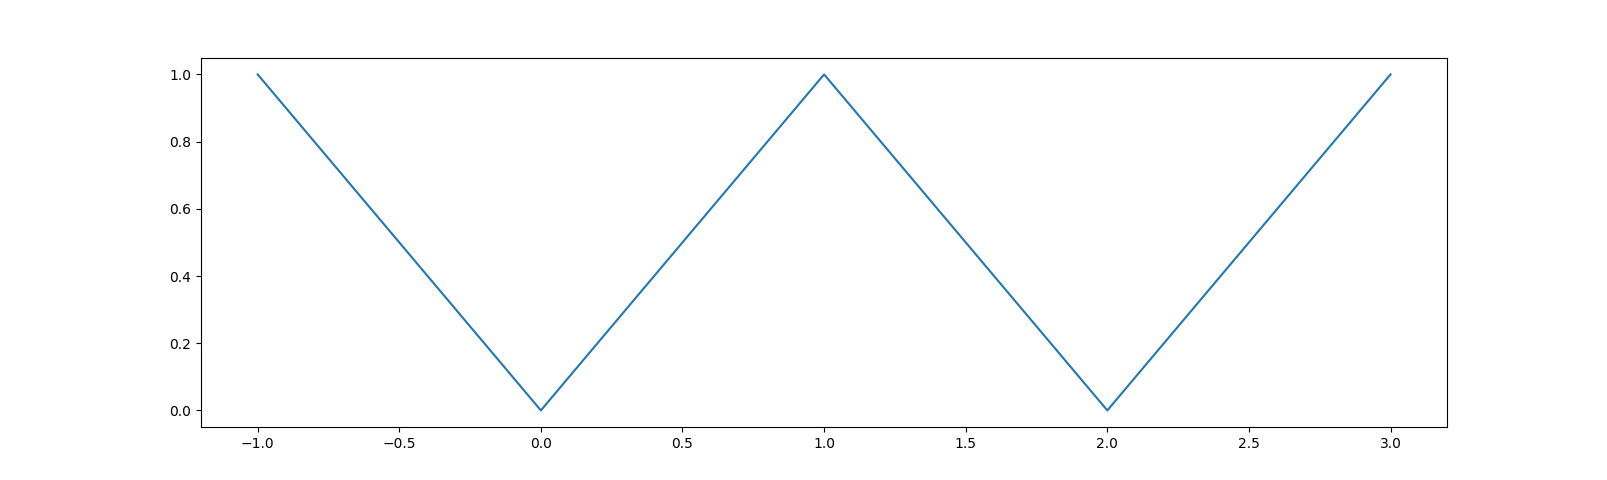
\includegraphics[scale=0.4]{TP19_triangle}
\end{center}
%--------------------------------------------------------------------------
%--------------------------------------------------------------------------
\begin{Exercise}\it
Écrire la fonction \type{triangle(x)} qui renvoie la valeur de la fonction 2-périodique égale à $|x|$ pour $x\in[-1;1]$.
\end{Exercise}
%--------------------------------------------------------------------------
\begin{Answer} 

Pour $x\in [2k-1;2k+1]$ on a $x-2k\in [-1;1]$ donc
$\text{triangle}(x)  = \text{triangle}(x-2k)  = |x-2k|$.

$2k-1\le x < 2k+1$ est équivalent à $k \le \frac{x+1}2 \le k+1$ ; on peut choisir $k = \big\lfloor \frac{x+1}2 \big\rfloor$.
    
\begin{lstlisting}
def triangle(x):
    k = floor((x+1)/2)
    return abs(x-2*k)
\end{lstlisting}
\end{Answer}
%--------------------------------------------------------------------------
%--------------------------------------------------------------------------
\begin{Exercise}\it
Représenter sur un même graphe la fonction triangle et les sommes partielles, $S_n(f)$, de sa série de Fourier pour $n\in \{1, 2, 3, 5, 20\}$ sur l'intervalle $[-1;3]$.
\end{Exercise}
%--------------------------------------------------------------------------
\begin{Answer}
\begin{lstlisting}
a = -1
b = 3
n = 1000
pas  = (b-a)/n
X = [a + k*pas for k in range(n+1)]
Y = [triangle(x) for x in X]
plt.plot(X, Y)

A = liste_a(triangle, 20, 2)
B = liste_b(triangle, 20, 2)

for N in [1, 2, 3, 5, 20]:
    Y = [somme_Fourier(A[ : N+1], B[ : N+1], 2, x) for x in X]
    plt.plot(X, Y, label="Somme d'ordre {}".format(N))
plt.legend()
plt.show()
\end{lstlisting}
Comme la fonction est paire les coefficients $b_n$ sont tous nuls.

De plus les coefficients $a_{2p}$ sont nuls aussi pour $p\ge 1$ ; il n'y a pas de différence entre $S_1(f)$ et $S_2(f)$.
\begin{center}
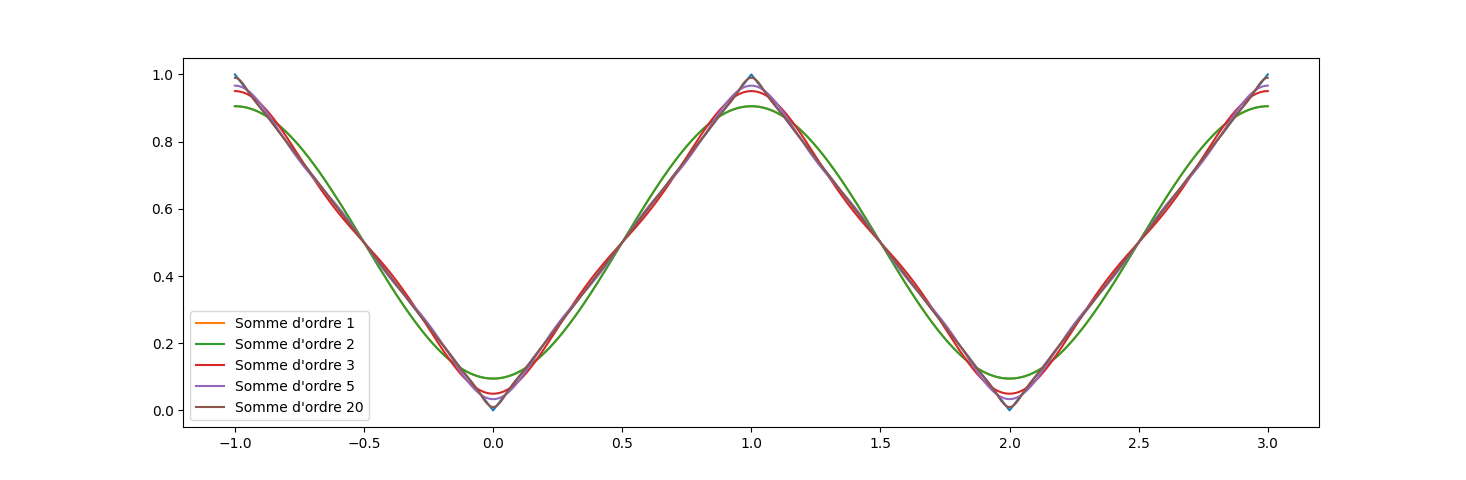
\includegraphics[scale=0.4]{TP/Images/TP19_triangle_Sn.png}
\end{center}
\end{Answer}
%--------------------------------------------------------------------------
%--------------------------------------------------------------------------
\subsection{Signal rectangulaire}
%--------------------------------------------------------------------------
%--------------------------------------------------------------------------
\begin{center}
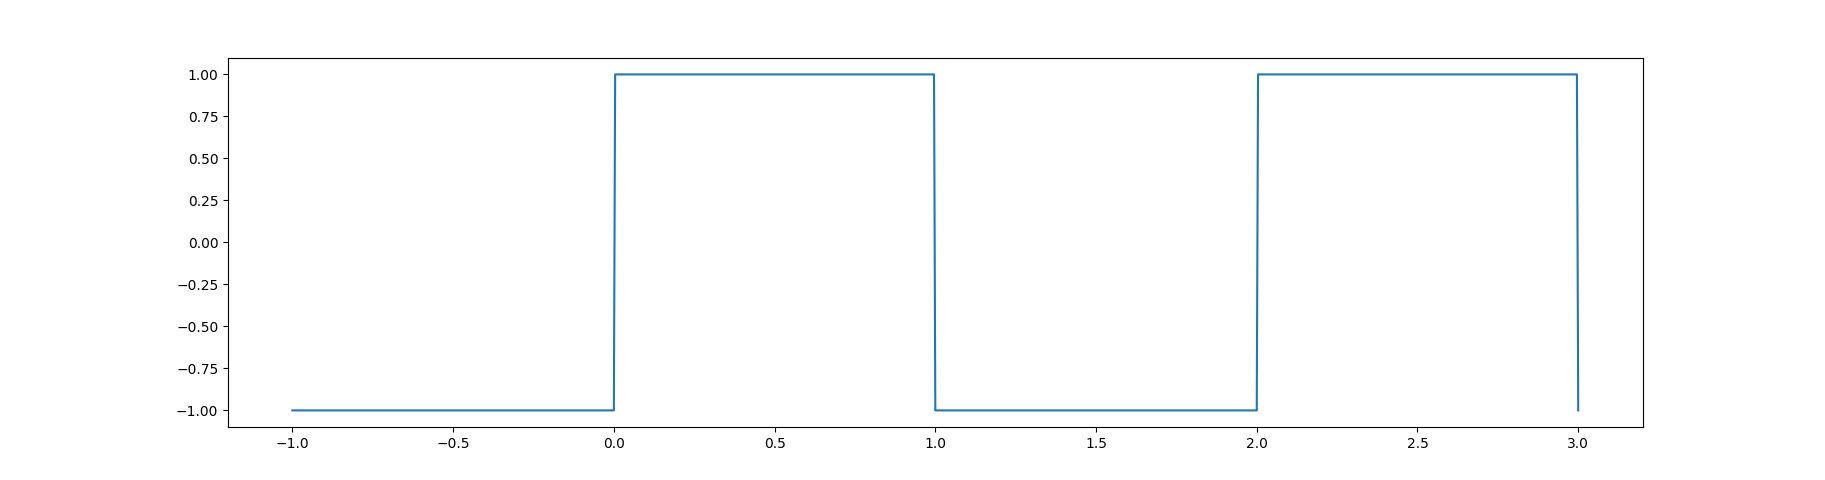
\includegraphics[scale=0.3]{TP/Images/TP19_rectangle.png}
\end{center}
%--------------------------------------------------------------------------
%--------------------------------------------------------------------------
\begin{Exercise}\it
Écrire la fonction \type{rectangle(x)} qui renvoie la valeur de la fonction 2-périodique égale à $1$ sur $]0;1[$, à  $-1$ sur $]-1;1[$ et à 0 aux points de $\Z$.
\end{Exercise}
%--------------------------------------------------------------------------
\begin{Answer} 

Pour $x\in [2k-1;2k+1]$ on a $x-2k\in [-1;1]$ donc
$\text{triangle}(x)  = \text{triangle}(x-2k)  = |x-2k|$.

$2k-1\le x < 2k+1$ est équivalent à $k \le \frac{x+1}2 \le k+1$ ; on peut choisir $k = \big\lfloor \frac{x+1}2 \big\rfloor$.
    
\begin{lstlisting}
def rectangle(x):
    k = floor((x+1)/2)
    if 0 < x - 2*k < 1:
        return 1
    elif -1 < x - 2*k < 0:
        return -1
    else:
        return 0
\end{lstlisting}
\newpage
\end{Answer}
%--------------------------------------------------------------------------
%--------------------------------------------------------------------------
\begin{Exercise}\it
Représenter sur un même graphe la fonction rectangle et les sommes partielles, $S_n(f)$, de sa série de Fourier pour $n\in \{1, 5, 10, 20, 50\}$ sur l'intervalle $[-1;3]$.
\end{Exercise}
%--------------------------------------------------------------------------
\begin{Answer}
\begin{lstlisting}
a = -1
b = 3
n = 1000
pas  = (b-a)/n
X = [a + k*pas for k in range(n+1)]
Y = [rectangle(x) for x in X]
plt.plot(X, Y)

A = liste_a(rectangle, 50, 2)
B = liste_b(rectangle, 50, 2)

for N in [1, 5, 10, 20, 50]:
    Y = [somme_Fourier(A[ : N+1], B[ : N+1], 2, x) for x in X]
    plt.plot(X, Y, label="Somme d'ordre {}".format(N))
plt.legend()
plt.show()
\end{lstlisting}
Comme la fonction est impaire les coefficients $a_n$ sont tous nuls.
\begin{center}
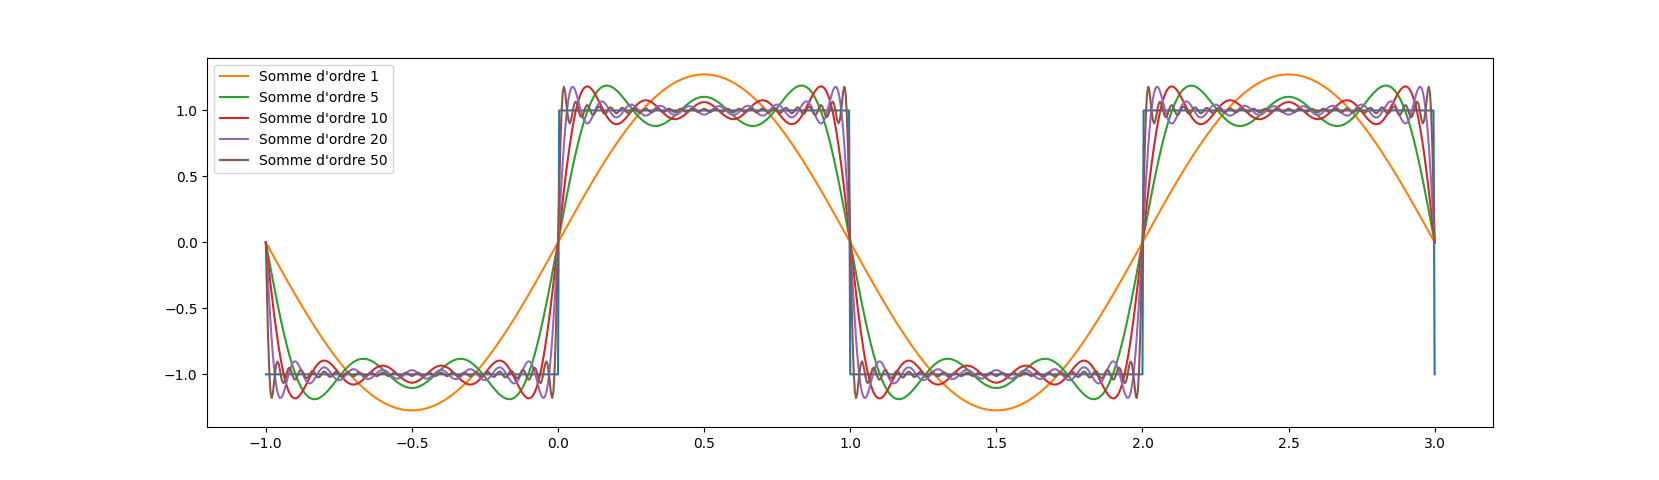
\includegraphics[scale=0.4]{TP/Images/TP19_rectangle_Sn.png}
\end{center}
\end{Answer}
%--------------------------------------------------------------------------
%--------------------------------------------------------------------------
On voit apparaître un dépassement incompressible de la valeur des sommes par rapport aux créneaux, c'est le phénomène de Gibbs.

On peut le faire disparaître en utilisant les sommes de Fejer, ce sont les moyennes des sommes de Fourier : 


\[F_N(f)(t) =   a_0 + \sum_{n=1}^{N} \bigl(a_n\cos(n\omega t) + b_n\sin(n\omega t)\bigr)\left(1 - \frac n{N+1}\right)\]

%--------------------------------------------------------------------------
%--------------------------------------------------------------------------
\begin{Exercise}\it
Représenter sur un même graphe la fonction rectangle et les sommes partielles, $S_n(f)$, de sa somme de Fejer pour $n\in \{1, 5, 10, 20, 50\}$ sur l'intervalle $[-1;3]$.
\end{Exercise}
%--------------------------------------------------------------------------
\begin{Answer}
\begin{lstlisting}
def somme_Fejer(A, B, T, x):
    N = len(A)
    s = 0
    w = 2*pi/T
    for n in range(N):
        s = s + (A[n]*cos(n*w*x) + B[n]*sin(n*w*x))*(1-n/N)
    return s
\end{lstlisting}
\newpage
\begin{lstlisting}
a = -1
b = 3
n = 1000
pas  = (b-a)/n
X = [a + k*pas for k in range(n+1)]
Y = [rectangle(x) for x in X]
plt.plot(X, Y)

A = liste_a(rectangle, 50, 2)
B = liste_b(rectangle, 50, 2)

for N in [1, 5, 10, 20, 50]:
    Y = [somme_Fejer(A[ : N+1], B[ : N+1], 2, x) for x in X]
    plt.plot(X, Y, label="Somme d'ordre {}".format(N))
plt.legend()
plt.show()
\end{lstlisting}
\begin{center}
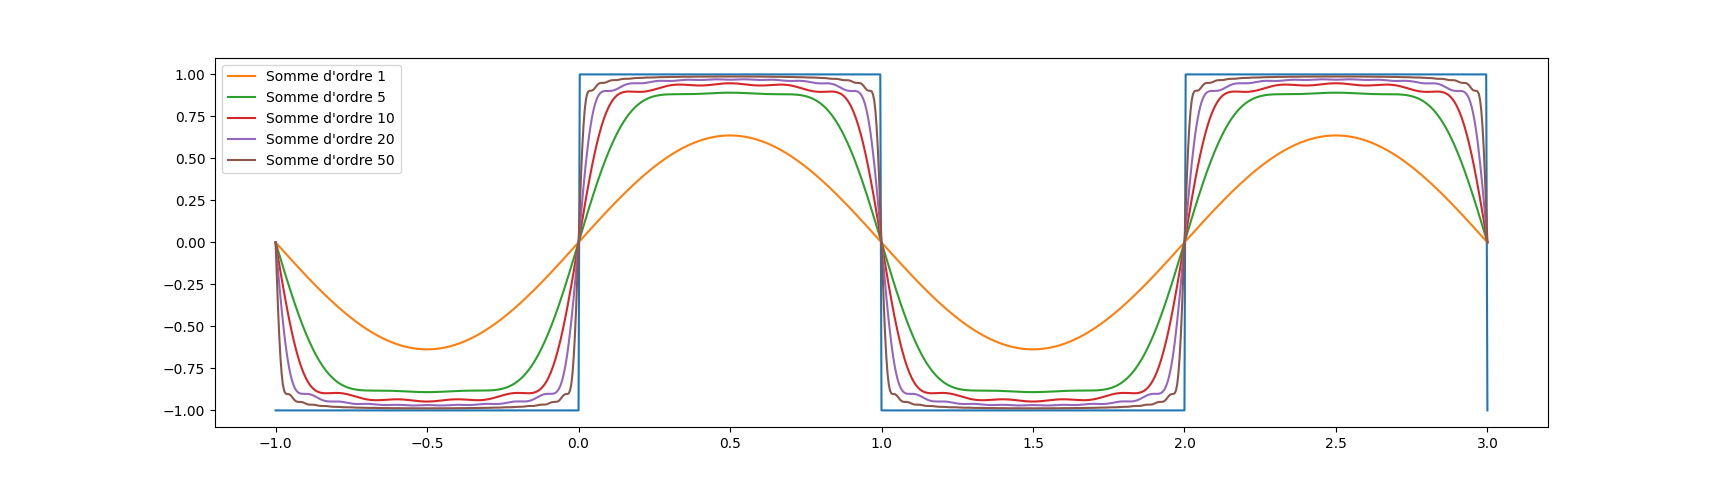
\includegraphics[scale=0.4]{TP/Images/TP19_rectangle_Fejer.png}
\end{center}
\end{Answer}
%--------------------------------------------------------------------------
%--------------------------------------------------------------------------
